\documentclass[../main.tex]{subfiles}
\graphicspath{{\subfix{../images/}}}
\begin{document}

% \subsubsection{Camera to LiDAR Extrinsic Calibration} \label{camLidar_calib}

Camera–LiDAR calibration begins by positioning a planar checkerboard target within both the LiDAR field of view and the camera image.  
The target’s physical dimensions in the LiDAR frame $(X_L, Y_L, Z_L)$ are matched to corresponding pixel coordinates $(u,v)$ in the image, yielding an initial estimate of the rigid transformation between sensor frames.  
A full derivation of this mapping is given in Appendix~\ref{img_tform}, and an example is shown in Figure~\ref{fig:calib_check}.

Initial calibration is performed using software such as the MATLAB LiDAR Calibration tool \cite{matlab_calibration}.  
Further refinement can be achieved either through iterative manual adjustment or by applying an \ac{ICP} algorithm, which minimizes point-to-plane error between the LiDAR point cloud and the camera-projected checkerboard corners.  
This approach produces a coarse transformation $_{C}^{L}\mathbf{T}$ adequate for accurate projection of LiDAR points into the image frame.

Manual fine-tuning may then be conducted by aligning prominent environmental features—such as walls, trees, and fences—visible in both modalities.  
This visual refinement yields sub-degree rotational and centimeter-level translational precision, sufficient for high-accuracy sensor fusion and object-detection tasks.  
In some cases, minor adjustments to the camera intrinsics are also necessary to compensate for small propagated errors.

% \begin{figure}[htbp]
% \centering
% \makebox[\textwidth][c]{
%     \begin{subfigure}[t]{0.44\textwidth}
%         \centering
%         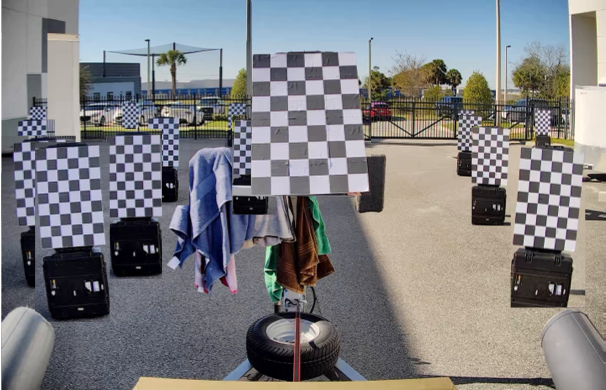
\includegraphics[width=\textwidth]{Images/checkerboard.png}
%         \caption{Composite image of multiple checkerboard target locations.}
%         \label{fig:checkerboard}
%     \end{subfigure}
%     \hspace{2em}
%     \begin{subfigure}[t]{0.44\textwidth}
%         \centering
%         \includegraphics[width=\textwidth]{Images/LiDAR_calib.png}
%         \caption{Composite of checkerboard locations in the LiDAR reference frame.}
%         \label{fig:LiDAR_calib}
%     \end{subfigure}
% }
% \caption{Checkerboard targets used for camera intrinsic (left) and LiDAR extrinsic (right) calibration. Red dots mark detected corner points transformed into the LiDAR frame using the initial extrinsic estimate.}
% \label{fig:camLidar_calib}
% \end{figure}


\end{document}